\section{The Fibonacci sequence}

\subsection{Objective}
Write an assembly program to generate the numbers of the Fibonacci series.


\subsection{Implementation}

The Fibonacci sequence is defined as follows:

\begin{align*}
	 & F_0 = 0                 \\
	 & F_1 = 1                 \\
	 & F_n = F_{n-1} + F_{n-2}
\end{align*}

\subsubsection{Assembly code}

\asmcode{./code/8086/fib.asm}

\subsection{Output}

\begin{figure}[h]
	\centering
	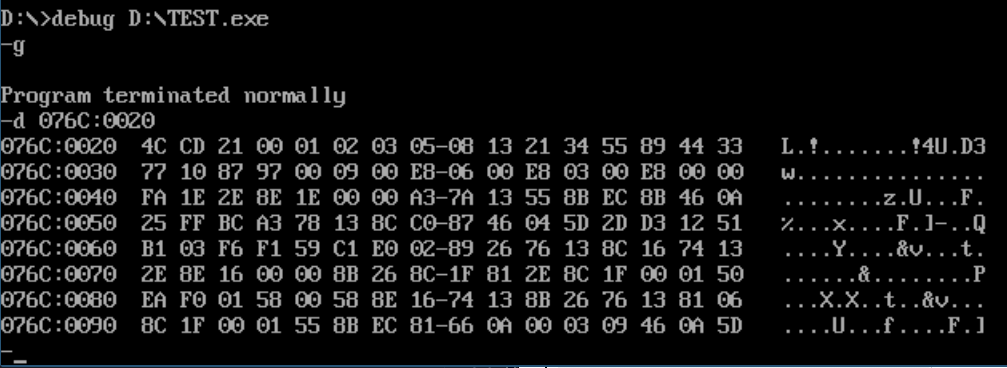
\includegraphics[width=0.8\textwidth]{./res/practicals/fib.png}
	\caption{Output of the program}
	\label{fig:fibonacci}
\end{figure}
